\chapter{Descrizione e sintesi del progetto in VHDL}
Si procederà in questo capitolo alla descrizione in VHDL del progetto, alla sua sintesi ed alle simulazioni di alcuni casi significativi di funzionamento corretto, infine procedendo all'implementazione su diverse FPGA al fine di effettuare comparazione di risultati in termini di performance, area occupata e potenza dissipata.

\section{FPGA: struttura interna}
\newpage

\begin{figure}[H]
	\centering
	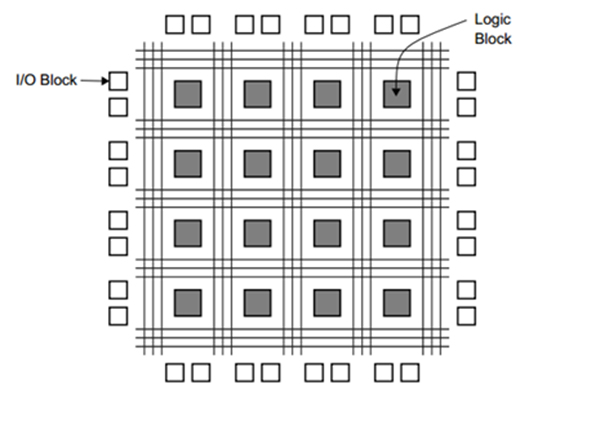
\includegraphics[scale=0.45]{3_FPGA_arch}
	\caption{Schema interno di una generica FPGA}
	\label{fig:fpga_architecture}
\end{figure}
La struttura di un FPGA è in generale costituita da una matrice di blocchi logici configurabili, detti CLB (Configurable Logic Blocks), connessi fra loro attraverso interconnessioni programmabili. Ai margini di tale matrice vi sono i blocchi di ingresso/uscita, detti IOB (Input Output Block). I CLB realizzano le funzioni logiche, l'insieme di interconnessioni li mette in comunicazione, mentre gli IOB si occupano dell'interfacciamento del circuito con l'esterno. All'interno di tale matrice sono presenti anche altri tipi di risorsa, come i DCM (Digital Clock Manager), che generano il segnale di clock, la rete che trasporta il segnale di clock dai flip-flop ai CLB ed altre risorse di calcolo, come ad esempio le ALU (Arithmetic Logic Unit), e risorse di memoria distribuita.

\subsection{CLB}
I blocchi CLB sono composti solitamente da due o quattro celle logiche (logic cell oppure slice), che eseguono le operazioni booleane. Ogni slice è solitamente composta da una o più LUT (Look-up Table) programmabili. Le LUT sono utilizzate per implementare funzioni booleane generalizzate, e sono solitamente accompagnate da un registro.
\begin{figure}[H]
	\centering
	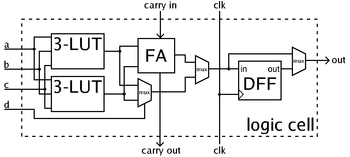
\includegraphics[scale=0.8]{3_FPGA_clb}
	\caption{Struttura di una slice}
	\label{fig:fpga_clb}
\end{figure}
\noindent
I CLB possono essere connessi fra loro, permettendo così di realizzare funzioni booleane complesse. Le LUT sono composte da una memoria SRAM da 16 bit e da un multiplexer a 4 ingressi: una volta configurate possono generare qualsiasi funzione logica a quattro ingressi ciascuna. Vi sono anche le interconnessioni relative alla logica di set/reset e chip enable, ai segnali di clock, e ai segnali provenienti dalle altre slice del dispositivo. La scelta di utilizzare LUT a soli quattro ingressi risiede nel fatto che la complessità di una LUT cresce esponenzialmente all'aumentare del numero di ingressi, e risulta dunque poco gestibile.zione dell'area occupata: CLB troppo grandi implicano che l'area necessaria per le interconnessioni locali superi quella risparmiata grazie al raggruppamento delle LUT contenute in esse. Lungo il perimetro dei blocchi logici vi sono infine i pin di ingresso e uscita, collegati all'interconnessione adiacente tramite transistor programmabili.

\section{Ambiente di sviluppo ISE Design Suite}
Per la descrizione hardware del progetto e la simulazione si è utilizzato il l'ambiente di sviluppo ISE Design Suite di Xilinx.
L'acronimo di ISE sta per Integrated Synthesis Environment ed è un software strettamente legato alle archietture di FPGA prodotte da Xilinx. ISE supporta la descrizione di moduli in linguaggio HDL (VHDL o Verilog) nonché consente l'implementazione di svariati moduli IP presenti nella libreria di sistema interna. Una volta completata la descrizione in linguaggio HDL si può procedere alla simulazione del progetto tramite il simulatore logico del software, denominato ISIM.
\begin{figure}[H]
	\centering
	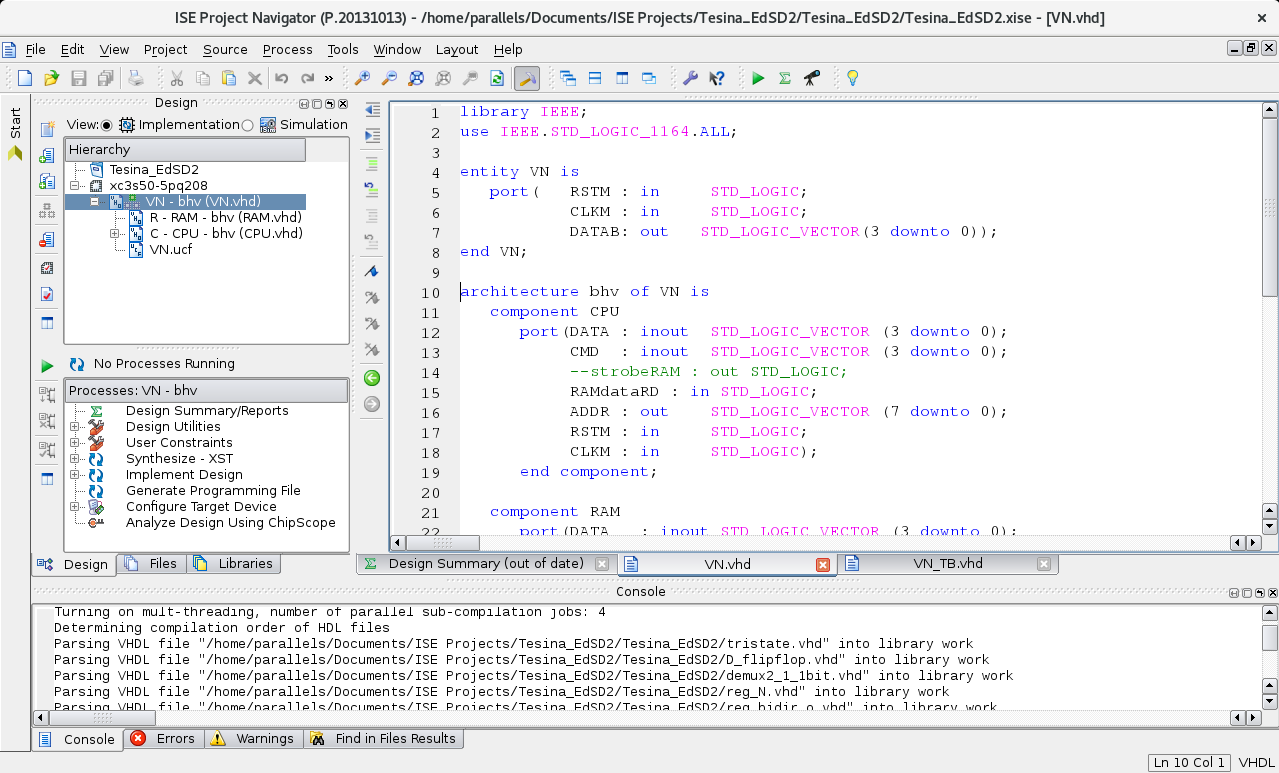
\includegraphics[scale=0.31]{3_ISE_interface}
	\caption{Interfaccia grafica di ISE}
	\label{fig:ise_interface}
\end{figure}
\par \bigskip
\begin{figure}[H]
	\centering
	\includegraphics[scale=0.31]{3_ISE_isim}
	\caption{Ambiente di simulazione ISIM}
	\label{fig:ise_isim}
\end{figure}
\noindent
Il processo di design e sintesi di un progetto su scheda FPGA si compone delle seguenti fasi:
\begin{itemize}
	\item \textbf{Descrizione} del circuito logico in linguaggio HDL (VHDL, VERILOG).
	\item \textbf{Sintesi} del circuito da descrizione hardware a netlist, ovvero l'insieme delle componenti logiche e le interconnessioni che realizzano il circuito logico descritto.
	\item \textbf{Simulazione behavioural}: verifica del funzionamento logico dell'hardware descritto.
	\item \textbf{Place \& Route}: Implementazione dell'harware descritto su FPGA. In questa fase tutti i componenti vengono fisicamente predisposti ad essere piazzati sulla scheda e, conseguentemente, il sistema prende effettivamente conoscenza di tutti i ritardi dovuti alle interconnessioni fisiche tra i vari blocchi descritti.
	\item \textbf{Simulazione post P\&R} che consente di simulare il layout fisico del progetto.
	\item Generazione del \textbf{bitstream}, ovvero di un file che contiene la descrizione digitale del posizionamento delle componenti sulla scheda.
	\item \textbf{Caricamento} sulla scheda per la finalizzazione del progetto.
\end{itemize}

\section{Descrizione in VHDL}
Una volta proceduto alla scrittura dei blocchi \textquotedblleft fondamentali" come tri-state e flip-flop, si è proceduto con un approccio bottom-up alla descrizione dell'intero progetto. Dal punto di vista \textquotedblleft gerarchico" il sistema è visto come un insieme di componenti annidati.
\begin{figure}[H]
	\centering
	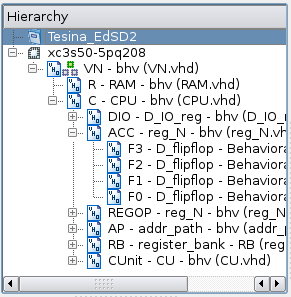
\includegraphics[scale=0.5]{3_ise_hierarchy}
	\caption{Visione gerarchica del sistema}
	\label{fig:ise_hierarchy}
\end{figure}
\noindent
Nella figura numero \ref{fig:ise_hierarchy}, ad esempio, il componente \textit{ACC} è definito come un insieme di 4 \textit{D\_flipflop} e fa parte del sistema denominato \textit{CPU}, a sua volta facente parte del sistema \textquotedblleft top-module" denominato VN.

\subsection{Top Module}
Il sistema dall'esterno è visto come un blocchetto denominato VN, al cui interno sono presenti i sottosistemi di RAM e CPU. È connesso esternamente col mondo esterno tramite un bus dati bidirezionale, e due segnali di ingresso relativi al CLOCK e RESET.
\begin{figure}[H]
	\centering
	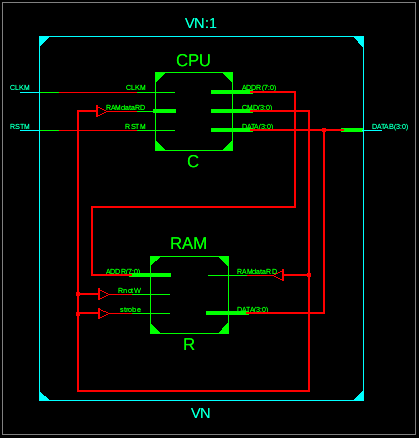
\includegraphics[scale=0.6]{3_ise_topmodule}
	\caption{Schema RTL del blocco top-module denominato VN}
	\label{fig:ise_topmodule}
\end{figure}
\noindent
Internamente, come nella visione gerarchica dell'architettura di Von Neumann vista nella sezione introduttiva e schematizzata in Figura \ref{fig:ist_0}, sono presenti i due sottoblocchi principali (escludendo il blocco di I/O) connessi tramite bus differenziato per dati, indirizzi e comandi.

\subsection{RAM}
La RAM assume un ruolo fondamentale in quanto è da essa che programmi e dati vengono prelevati. È concettualmente divisa in due aree, area dati ed area programmi, ed è indirizzata tramite bus ADDR a 2N bit.
La visione schematica RTL della sua descrizione VHDL è la seguente:
\begin{figure}[H]
	\centering
	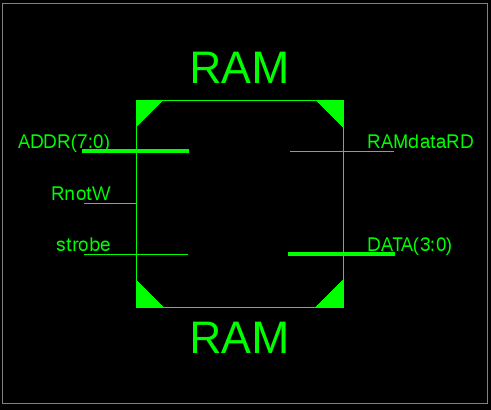
\includegraphics[scale=0.5]{3_ise_ram}
	\caption{Schema RTL del blocco RAM descritto in VHDL}
	\label{fig:ise_ram}
\end{figure}
\noindent
All'interno di essa è possibile memorizzare programmi e dati. Nella seguente immagine un esempio dell'area programmi contenente i valori di un semplice programma di test come verrebbero scritti dalla traduzione in linguaggio macchina del codice assembler.
\begin{figure}[H]
	\centering
	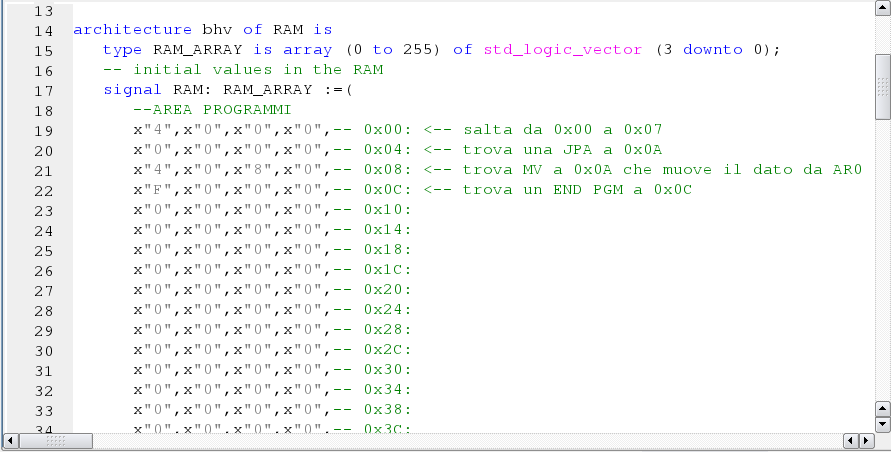
\includegraphics[scale=0.4]{3_ise_ram1}
	\caption{Descrizione harware del contenuto della RAM}
	\label{fig:ise_ram_code}
\end{figure}
\noindent
Mentre invece il processo che regola la selezione della lettura o scrittura nella memoria è riportato nella seguente Figura \ref{fig:ise_ram_process}.
\begin{figure}[H]
	\centering
	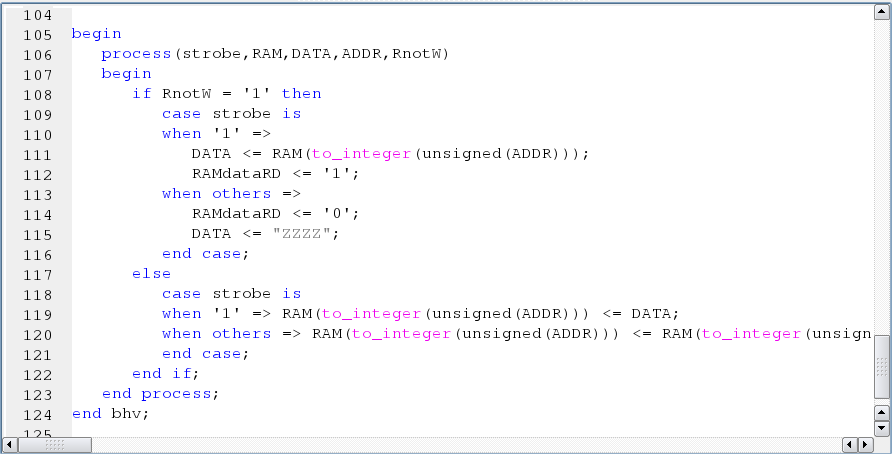
\includegraphics[scale=0.4]{3_ise_ram_proc}
	\caption{Descrizione harware del processo di selezione lettura/scrittura parola da memoria}
	\label{fig:ise_ram_process}
\end{figure}

%\newpage
\subsection{CPU}
\begin{figure}[H]
	\centering
	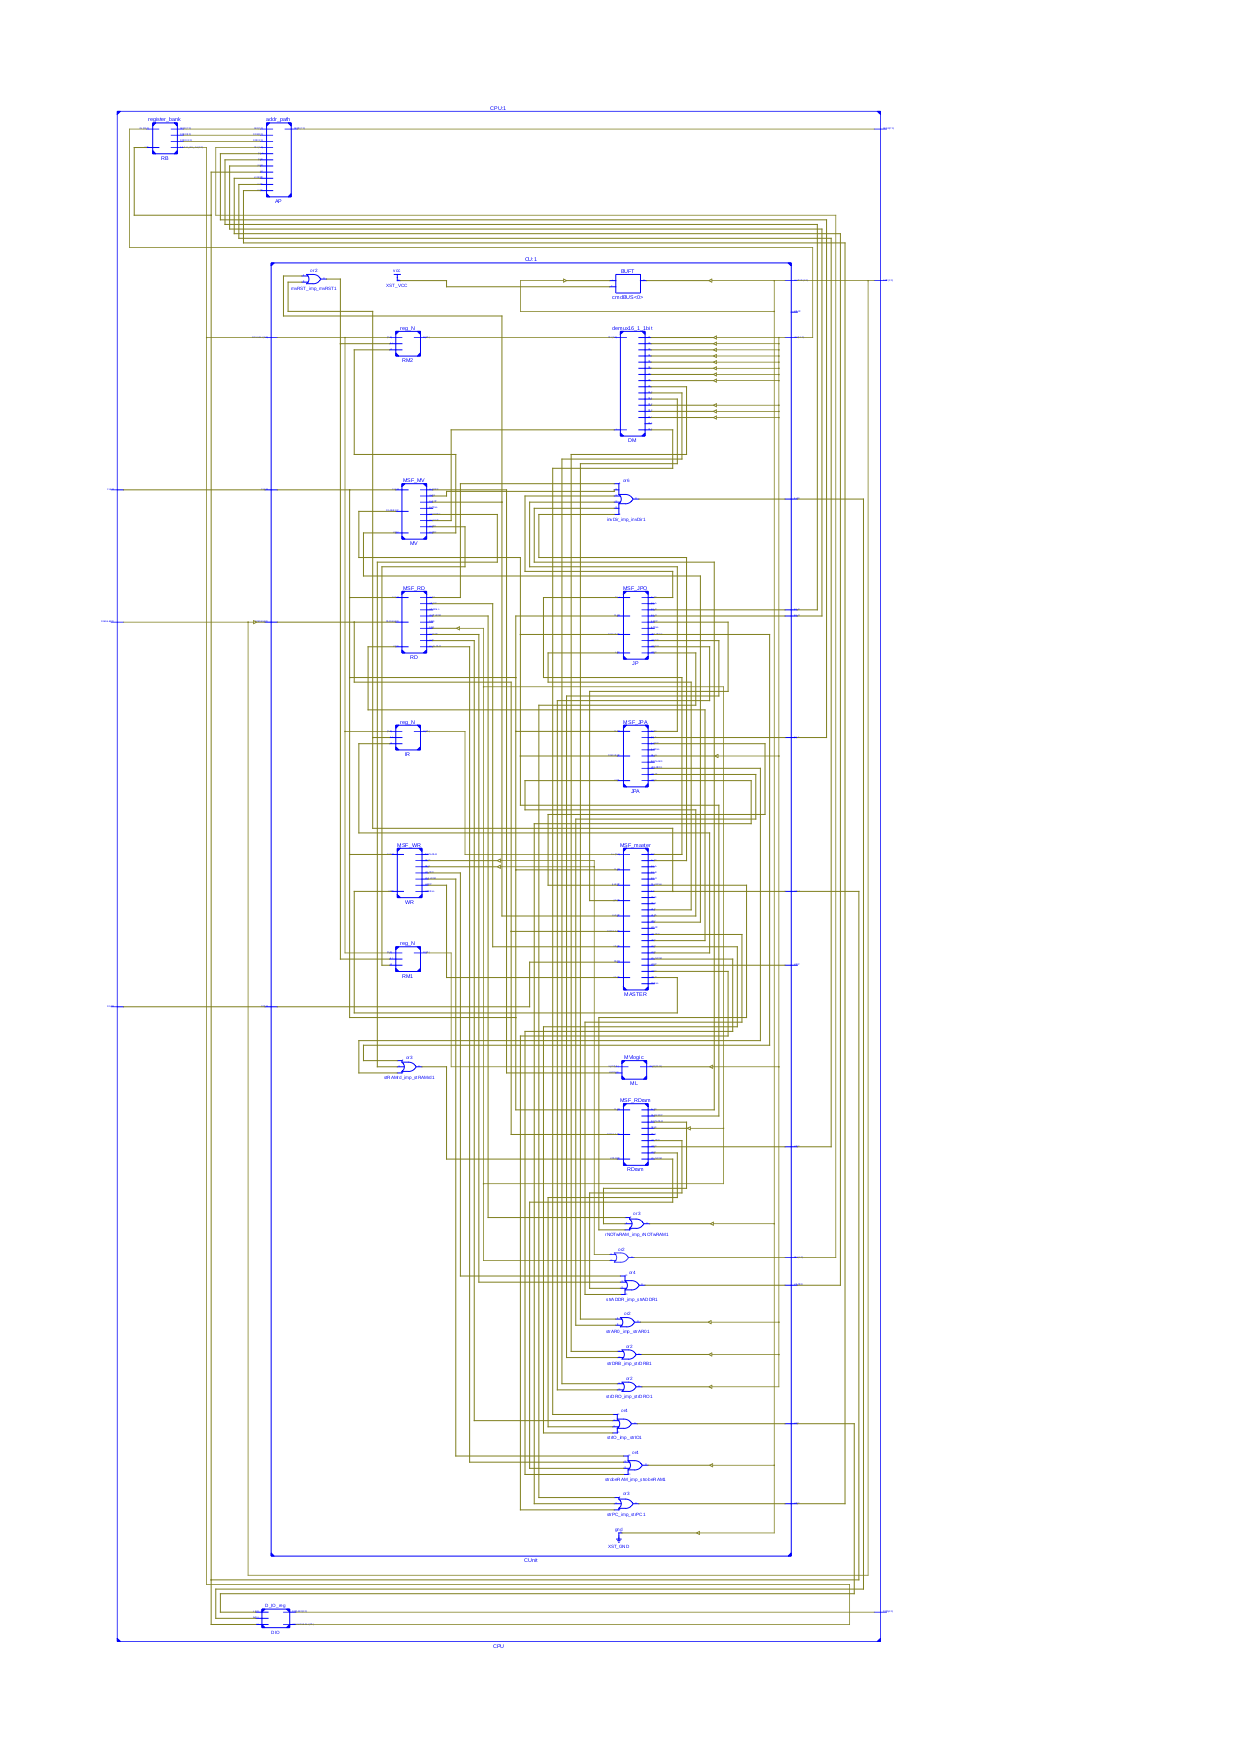
\includegraphics[scale=0.6]{3_ise_internal}
	\caption{Visione RTL dello schema interno del blocco CPU con esplosione del blocco di controllo CU}
	\label{fig:ise_internal}
\end{figure}
\noindent
All'interno della CPU trovano posto le unità istanziate nello schema di seconda istanziazione riportato in Sezione \ref{seconda_ist}. Parte del codice VHDL che descrive tale sottoblocco è il seguente.
\begin{figure}[H]
	\centering
	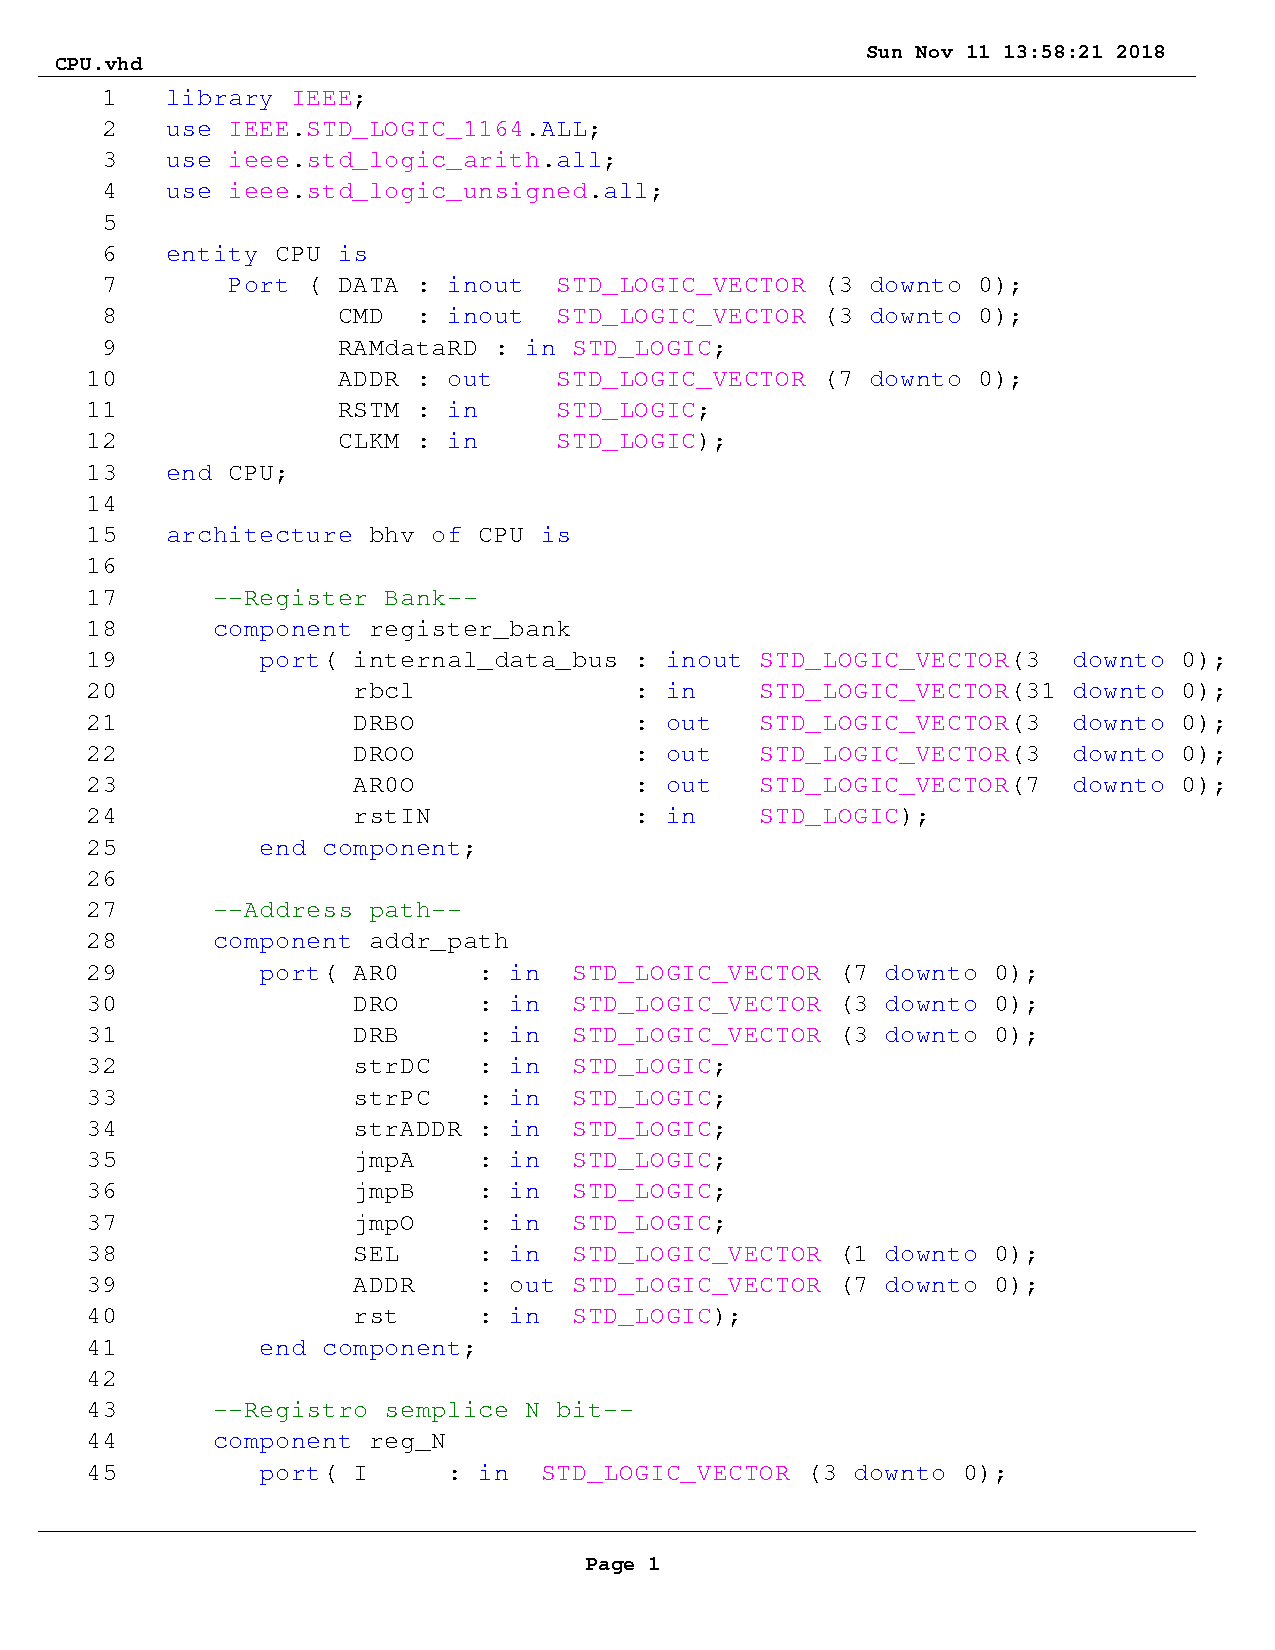
\includegraphics[scale=0.62]{3_ise_vhdl_cpu}
	\caption{Descrizione del blocco CPU}
	\label{fig:ise_vhdl_cpu}
\end{figure}
\noindent
Infine parte della descrizione della MSF MASTER di gestione operazioni.
\begin{figure}[H]
	\centering
	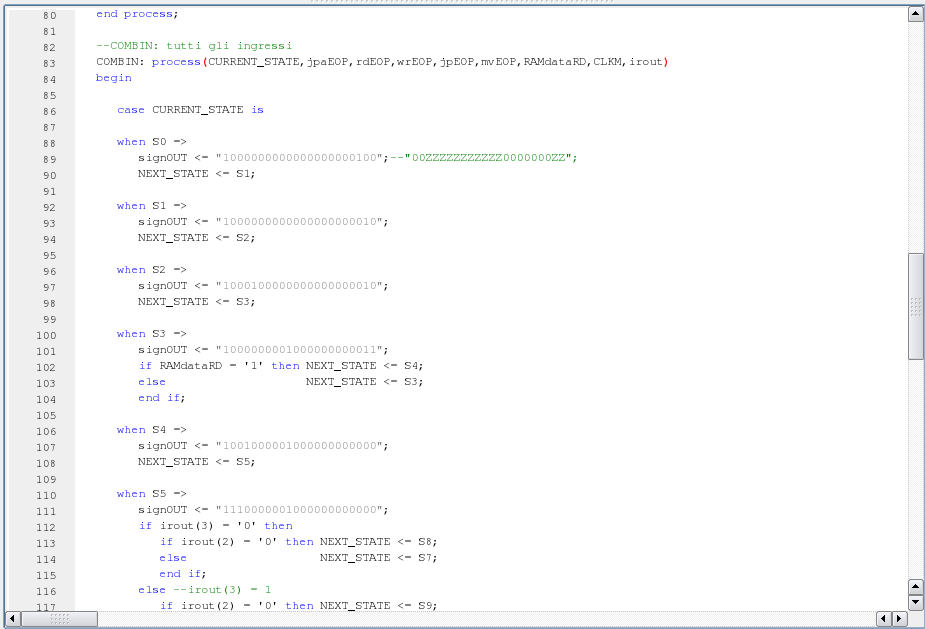
\includegraphics[scale=0.42]{3_ise_master}
	\caption{Parte del codice VHDL relativo alla descrizione della MSF MASTER}
	\label{fig:ise_master_msf}
\end{figure}

\subsection{Simulazioni}
Dopo aver sintetizzato tutto il sistema si è proceduto alle simulazioni post Place\&Route per garantire che i risultati delle simulazioni coincidano con i risultati effettivamente ricavati dal sistema fisico. Si è proceduto dapprima con la simulazione dei singoli blocchi per garantirne la funzionalità a priori ed, in seguito, alla simulazione completa di più esempi di programma. A seguire alcune delle simulazioni effettuate.
\begin{figure}[H]
	\centering
	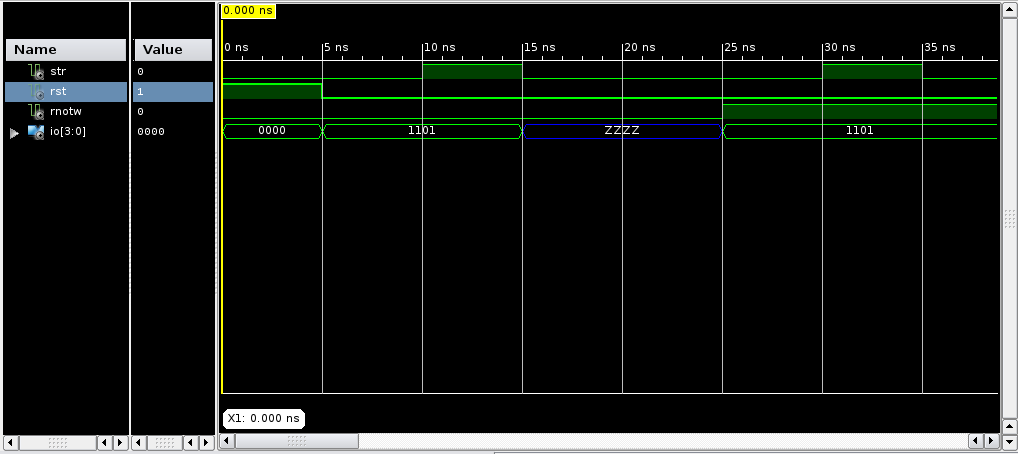
\includegraphics[scale=0.4]{3_sim_bidir}
	\caption{Simulazione del funzionamento dei registri bidirezionali. Si può notare l'applicazione di un dato esterno sul bus, lo strobe del dato, e l'inversione dell'uscita del registro che pilotando ora il bus porta in uscita il valore salvato. Infine la reiezione allo strobe quando il registro è in fase di lettura.}
	\label{fig:sim_bidir}
\end{figure}
\begin{figure}[H]
	\centering
	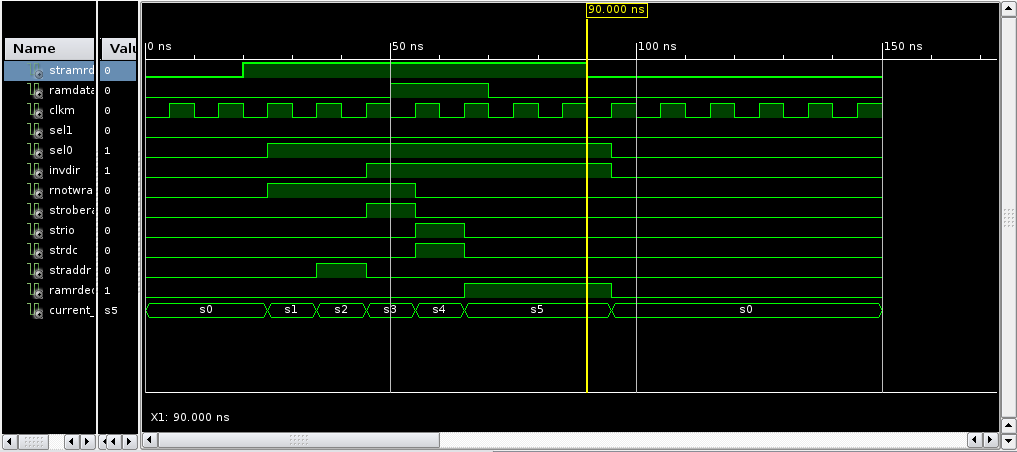
\includegraphics[scale=0.4]{3_sim_msf_rdram}
	\caption{Simulazione dell'evoluzione dello stato e dei segnali della MSF RD\_RAM che si occupa del prelievo dei dati dalla memoria RAM esterna. Si può notare l'evoluzione degli stati in risposta alle operazioni di lettura in memoria.}
	\label{fig:sim_msf_rdram}
\end{figure}
\begin{figure}[H]
	\centering
	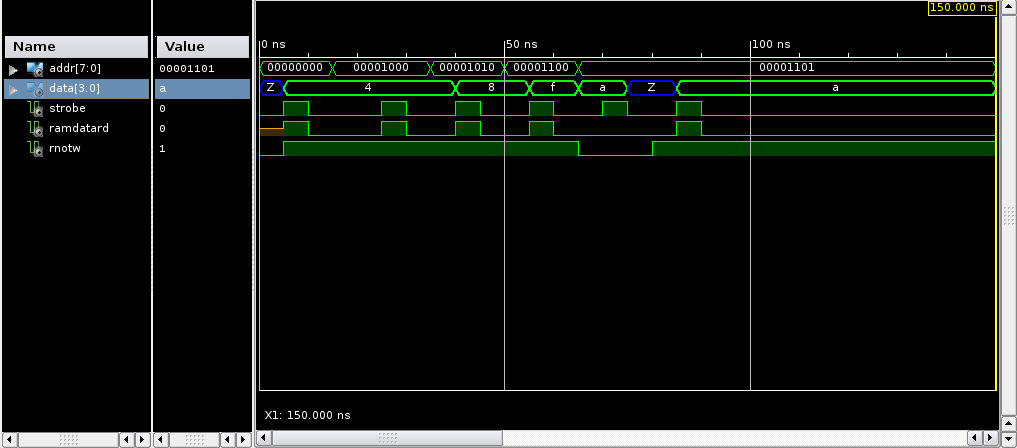
\includegraphics[scale=0.4]{3_sim_ram}
	\caption{Simulazione di lettura e scrittura sulla memoria. Come si può notare quando il segnale R/$\overline{W}$ è 0 la memoria salva il dato nella locazione imposta (nell'esempio 0x0D) e lo fornisce in uscita una volta che il segnale torna ad 1.}
	\label{fig:sim_ram}
\end{figure}
\noindent
Infine, testati gli apparati singolarmente si è proceduto alla scrittura del seguente programma di test.
\begin{lstlisting}[frame=single] 
0x00	JPA 0, 7		% salta all'indirizzo 0x07
0x07	NOP				% nessuna operazione
0x08	JBO 8,6		% salta a 8+6=14 (0x0E)
0x0E	NOP		      %nessuna operazione
0x0F	MV AR0,ACC		%copia il valore di AR0 in ACC
0x10	END		%termina l'esecuzione del programma
\end{lstlisting}
\begin{figure}[H]
	\centering
	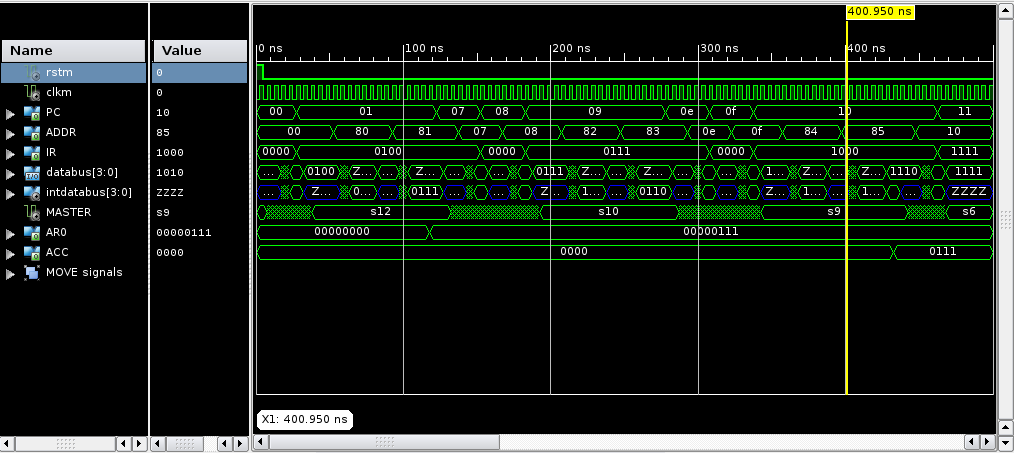
\includegraphics[scale=0.4]{3_sim_pgm}
	\caption{Simulazione del programma elencato. Si possono notare gli stati della macchina MASTER e le istruzioni presenti in IR pari a quanto scritto nel programma. Gli stati più lunghi della MASTER corrispondono alle attese di fine operazione degli slave.}
	\label{fig:sim_pgm}
\end{figure}
Nella macchina master gli stati relativi all'avvio e l'attesa di uno slave sono:
\begin{itemize}
	\item S8: NOP
	\item S9: slave MOVE
	\item S10: slave JBO
	\item S11: slave JPO
	\item S12: slave JPA
	\item S13: slave WR
	\item S14: slave RD
	\item S6: END PGM
\end{itemize}
Si può notare come questi coincidano nel caso dell'esecuzione del programma di Figura \ref{fig:sim_pgm}.

\section{Analisi dei risultati ottenuti}
Procedendo all'implementazione del progetto su di una FPGA fisica si analizzeranno di seguito i risultati. Le FPGA prese in considerazione sono le seguenti:
\begin{itemize}
	\item Spartan 3 - XC3S50
	\item Spartan 3 - XC3S1000
	\item Spartan 6 - XC6SLX75T
\end{itemize}
Il produttore fornisce le seguenti tabelle dove sono elencate le caratteristiche di tali FPGA.
\begin{figure}[H]
	\centering
	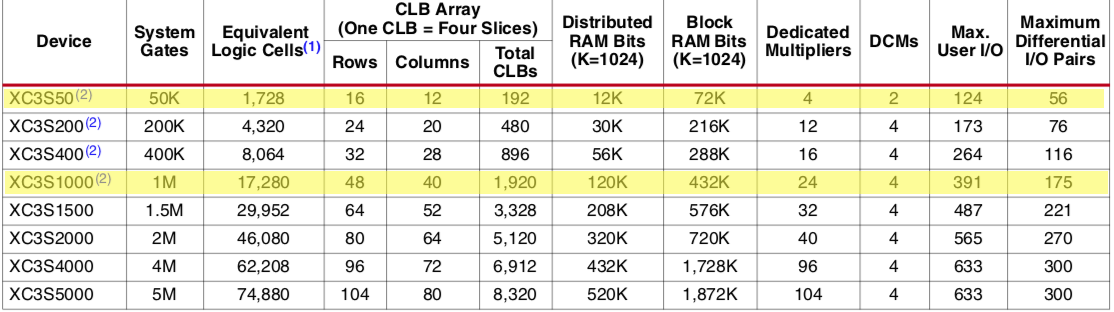
\includegraphics[scale=0.4]{3_sp3}
	\caption{Caratteristiche Xilinx Spartan 3.}
	\label{fig:spartan3}
\end{figure}
\begin{figure}[H]
\centering
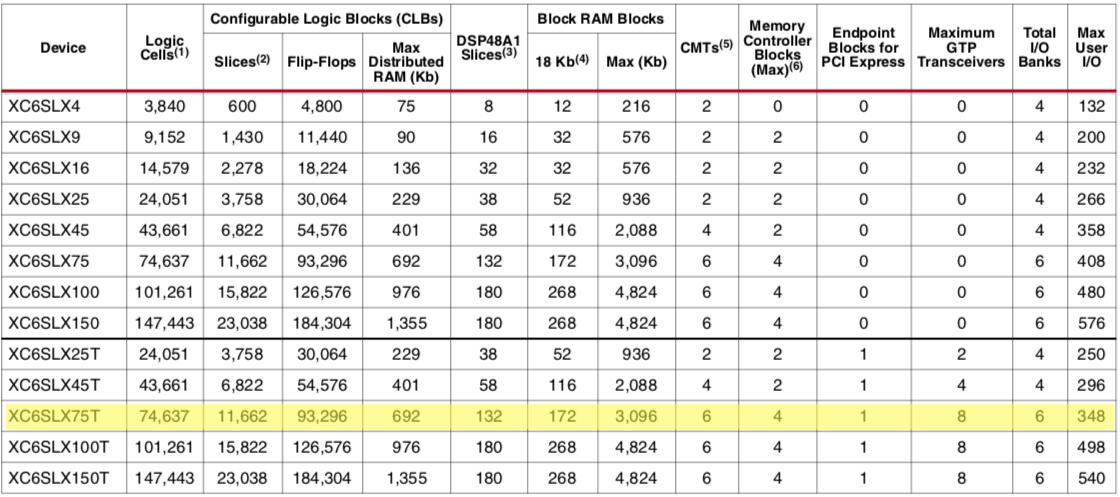
\includegraphics[scale=0.4]{3_sp6}
\caption{Caratteristiche Xilinx Spartan 6.}
\label{fig:spartan6}
\end{figure}
Si andranno ora a valutare i parametri ottenuti in fase di simulazione relativi a performance, area occupata e potenza dissipata.

\subsection{Performance}
Le performance temporali in termini di massima frequenza di clock ottenute a seguito della implementazione del progetto sulle FPGA prese in considerazione sono riassunte nella seguente tabella.
\begin{table}[H]
	\centering
	\fontsize{10}{18}\selectfont
	\begin{tabular}{|p{30mm}|p{30mm}|p{30mm}|p{30mm}|}
		\hline
		\multicolumn{1}{|c|}{\multirow{2}{*}{\textbf{{FPGA}}}} &
		\multicolumn{1}{c|}{\textbf{FPGA Features}} & 
		\multicolumn{2}{c|}{\textbf{Project features}} \\
		
		\cline{2-4}
		\multicolumn{1}{|c|}{} &
		\multicolumn{1}{c|}{\textit{Maximum frequency}} & 
		\multicolumn{1}{c|}{\textit{Minimum Period}} &
		\multicolumn{1}{c|}{\textit{Maximum Frequency}} \\
		
		\hline
		\multicolumn{1}{|c|}{Spartan 3 - XC3S50} &
		\multicolumn{1}{c|}{280 MHz} & 
		\multicolumn{1}{c|}{7.760 ns} &
		\multicolumn{1}{c|}{128.87 MHz (-54\%)} \\
		
		\hline
		\multicolumn{1}{|c|}{Spartan 3 - XC3S1000} &
		\multicolumn{1}{c|}{280 MHz} & 
		\multicolumn{1}{c|}{9.019 ns} &
		\multicolumn{1}{c|}{110.88 MHz (-60\%)} \\
		
		\hline
		\multicolumn{1}{|c|}{Spartan 6 - XC6SLX75T} &
		\multicolumn{1}{c|}{320 MHz} & 
		\multicolumn{1}{c|}{3.307 ns} &
		\multicolumn{1}{c|}{302.421 MHz (-6\%)}\\ \hline
		
	\end{tabular}
\caption{Comparazione dei ritardi e della massima frequenza di clock ammissibile.}
\end{table}
\noindent
Si può notare che nonostante la Spartan 3 XC3S50 abbia a disposizione minori risorse rispetto alla XC3S100 il routing ha fornito una frequenza di clock massima ammissibile maggiore. I risultati ottenuti sulla Spartan 6 - XC6SLX75T superano ampiamente i risultati ottenuti nella famiglia Spartan 3 a livello prestazionale.

\subsection{Area occupata}
I risultati ottenuti in termini di occupazione delle risorse disponibili nelle FPGA sono sintetizzati nella seguente tabella.
\begin{table}[H]
	\centering
	\fontsize{10}{18}\selectfont
	\begin{tabular}{|p{20mm}|p{13mm}|p{13mm}|p{13mm}|p{13mm}|p{13mm}|p{13mm}|}
		\hline
		\multicolumn{1}{|c|}{\multirow{2}{*}{}} &
		\multicolumn{2}{c|}{\textbf{Spartan 3 - XC3S50}} & 
		\multicolumn{2}{c|}{\textbf{Spartan 3 - XC3S1000}} & 
		\multicolumn{2}{c|}{\textbf{Spartan 6 - XC6SLX75T}} \\
		
		\cline{2-7} &
		\multicolumn{1}{c|}{\textbf{Usate}} & 
		\multicolumn{1}{c|}{\textbf{Disponibili}} &
		\multicolumn{1}{c|}{\textbf{Usate}} & 
		\multicolumn{1}{c|}{\textbf{Disponibili}} &
		\multicolumn{1}{c|}{\textbf{Usate}} & 
		\multicolumn{1}{c|}{\textbf{Disponibili}} \\
		
		\hline
		\multicolumn{1}{|c|}{Number of Slices} &
		\multicolumn{1}{|c|}{\multirow{2}{*}{151 (9\%)}} &
		\multicolumn{1}{|c|}{\multirow{2}{*}{1.536}} &
		\multicolumn{1}{|c|}{\multirow{2}{*}{151 (1\%)}} &
		\multicolumn{1}{|c|}{\multirow{2}{*}{15.360}} &
		\multicolumn{1}{|c|}{\multirow{2}{*}{144 (1\%)}} &
		\multicolumn{1}{|c|}{\multirow{2}{*}{93.296}} \\
		%\cline{2-7}
		\multicolumn{1}{|c|}{flip-flop} &&&&&&\\
		
		\hline
		\multicolumn{1}{|c|}{Number of 4-input} &
		\multicolumn{1}{|c|}{\multirow{2}{*}{244 (15\%)}} &
		\multicolumn{1}{|c|}{\multirow{2}{*}{1.536}} &
		\multicolumn{1}{|c|}{\multirow{2}{*}{244 (1\%)}} &
		\multicolumn{1}{|c|}{\multirow{2}{*}{15.360}} &
		\multicolumn{1}{|c|}{\multirow{2}{*}{174 (1\%)}} &
		\multicolumn{1}{|c|}{\multirow{2}{*}{46.648}} \\
		%\cline{2-7}
		\multicolumn{1}{|c|}{LUTs} &&&&&&\\
		
		\hline
		\multicolumn{1}{|c|}{Number of bonded} &
		\multicolumn{1}{|c|}{\multirow{2}{*}{17 (13\%)}} &
		\multicolumn{1}{|c|}{\multirow{2}{*}{124}} &
		\multicolumn{1}{|c|}{\multirow{2}{*}{17 (9\%)}} &
		\multicolumn{1}{|c|}{\multirow{2}{*}{173}} &
		\multicolumn{1}{|c|}{\multirow{2}{*}{17 (4\%)}} &
		\multicolumn{1}{|c|}{\multirow{2}{*}{384}} \\
		%\cline{2-7}
		\multicolumn{1}{|c|}{IOBs} &&&&&&\\ \hline
		
	\end{tabular}
\end{table}
\noindent
Dunque, come era possibile aspettarsi, le FPGA aventi maggiori risorse hanno subito una minore occupazione di area.

\begin{figure}[H]
	\centering
	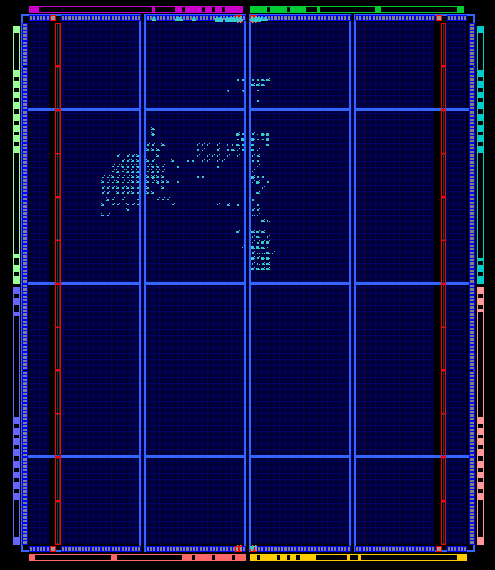
\includegraphics[scale=0.55]{3_ise_area}
	\caption{Esempio di routing su FPGA Spartan 3 - XC3S1000}
	\label{fig:area_occupata}
\end{figure}

\subsection{Power}
Nella tabella seguente un riepilogo dei consumi.
\begin{table}[H]
	\centering
	\fontsize{10}{18}\selectfont
	\begin{tabular}{|p{30mm}|p{30mm}|p{30mm}|p{30mm}|}
		\hline
		\multicolumn{1}{|c|}{} &
		\multicolumn{1}{c|}{\textbf{Spartan 3 - XC3S50}} & 
		\multicolumn{1}{c|}{\textbf{Spartan 3 - XC3S1000}} & 
		\multicolumn{1}{c|}{\textbf{Spartan 6 - XC6SLX75T}} \\
		
		\hline
		\multicolumn{1}{|c|}{Speed grade} &
		\multicolumn{1}{c|}{-5} & 
		\multicolumn{1}{c|}{-5} & 
		\multicolumn{1}{c|}{-3} \\
		
		\hline
		\multicolumn{1}{|c|}{Clock} &
		\multicolumn{1}{c|}{0.000} & 
		\multicolumn{1}{c|}{0.000} & 
		\multicolumn{1}{c|}{0.000} \\
		
		\hline
		\multicolumn{1}{|c|}{Logic} &
		\multicolumn{1}{c|}{0.000} & 
		\multicolumn{1}{c|}{0.000} & 
		\multicolumn{1}{c|}{0.000} \\
		
		\hline
		\multicolumn{1}{|c|}{Signals} &
		\multicolumn{1}{c|}{0.000} & 
		\multicolumn{1}{c|}{0.000} & 
		\multicolumn{1}{c|}{0.000} \\
		
		\hline
		\multicolumn{1}{|c|}{DSPs} &
		\multicolumn{1}{c|}{0.000} & 
		\multicolumn{1}{c|}{0.000} & 
		\multicolumn{1}{c|}{0.000} \\
		
		\hline
		\multicolumn{1}{|c|}{IOs} &
		\multicolumn{1}{c|}{0.000} & 
		\multicolumn{1}{c|}{0.000} & 
		\multicolumn{1}{c|}{0.000} \\
		
		\hline
		\multicolumn{1}{|c|}{Leakeage} &
		\multicolumn{1}{c|}{0.027} & 
		\multicolumn{1}{c|}{0.098} & 
		\multicolumn{1}{c|}{0.064} \\
		
		\hline
		\multicolumn{1}{|c|}{\textbf{TOTAL}} &
		\multicolumn{1}{c|}{0.027 W} & 
		\multicolumn{1}{c|}{0.098 W} & 
		\multicolumn{1}{c|}{0.064 W} \\ \hline
		
	\end{tabular}
	\caption{Comparazione delle massime potenze dissipate in W}
\end{table}

\section{Conclusioni}
Dunque i risultati ottenuti si possono sintetizzare nella seguente tabella.
\begin{table}[H]
	\centering
	\fontsize{10}{18}\selectfont
	\begin{tabular}{|p{30mm}|p{30mm}|p{30mm}|p{30mm}|}
		\hline
		\multicolumn{1}{|c|}{} &
		\multicolumn{1}{c|}{\textbf{Spartan 3 - XC3S50}} & 
		\multicolumn{1}{c|}{\textbf{Spartan 3 - XC3S1000}} & 
		\multicolumn{1}{c|}{\textbf{Spartan 6 - XC6SLX75T}} \\
		
		\hline
		\multicolumn{1}{|c|}{PERFORMANCE} &
		\multicolumn{1}{c|}{++} & 
		\multicolumn{1}{c|}{+} & 
		\multicolumn{1}{c|}{+++} \\
		
		\hline
		\multicolumn{1}{|c|}{AREA} &
		\multicolumn{1}{c|}{+++} & 
		\multicolumn{1}{c|}{++} & 
		\multicolumn{1}{c|}{+} \\
		
		\hline
		\multicolumn{1}{|c|}{POWER} &
		\multicolumn{1}{c|}{+} & 
		\multicolumn{1}{c|}{+++} & 
		\multicolumn{1}{c|}{++} \\ \hline
		
	\end{tabular}
	\caption{Comparazione risultati}
\end{table}
\noindent
Le prestazioni migliori si sono ottenute, in linea con quanto aspettato, sulla Spartan 6 che è risultata un buon compromesso a livello prestazionale registrando le migliori performance di Speed e di Area relativa alle risorse possedute.\\
Stranamente il tool ha fornito risultati migliori in termini di frequenza massima e potenza dissipata sulla più piccola Spartan3-XC3S50 rispetto alla sorella maggiore XC3S1000, probabilmente dovuto ad un cattivo settaggio del tool di Place\&Route.


\begin{table}[H]
	\centering
	\begin{tabular}{l|p{2cm}|}
		\cline{2-2} \multicolumn{1}{c|}{0x00} & \makebox[2cm][c]{\textbf{MV}}\\
		\cline{2-2} \multicolumn{1}{c|}{0x01} & \makebox[2cm][c]{\textbf{MV}}\\
		\cline{2-2} \multicolumn{1}{c|}{0x02} & \makebox[2cm][c]{\textbf{SUM}}\\
		\cline{2-2} \multicolumn{1}{c|}{0x03} & \makebox[2cm][c]{\textbf{MV}}\\
		\cline{2-2}
		\multicolumn{1}{c|}{\multirow{2}{*}{}} & \multicolumn{1}{c|}{\multirow{2}{*}{...}}\\
		& \\
		
		\cline{2-2} \multicolumn{1}{c|}{0x3F} & \makebox[2cm][c]{...}\\
		\cline{2-2} \multicolumn{0}{c|}{0x40} & \makebox[2cm][c]{DR1}\\
		\cline{2-2} \multicolumn{0}{c|}{0x41} & \makebox[2cm][c]{OP1}\\
		\cline{2-2} \multicolumn{0}{c|}{0x42} & \makebox[2cm][c]{DR2}\\
		\cline{2-2} \multicolumn{0}{c|}{0x43} & \makebox[2cm][c]{OP2}\\
		\cline{2-2} \multicolumn{0}{c|}{0x44} & \makebox[2cm][c]{ACC}\\
		\cline{2-2} \multicolumn{0}{c|}{0x45} & \makebox[2cm][c]{RIS}\\		\cline{2-2}
		\multicolumn{1}{c|}{\multirow{2}{*}{}} & \multicolumn{1}{c|}{\multirow{2}{*}{...}}\\
		& \\
		\cline{2-2} \multicolumn{1}{c|}{0xFF} & \makebox[2cm][c]{...}\\ \cline{2-2}
	\end{tabular}
	%\caption*{Organizzazione della memoria relativa al programma d'esempio }
\end{table}